    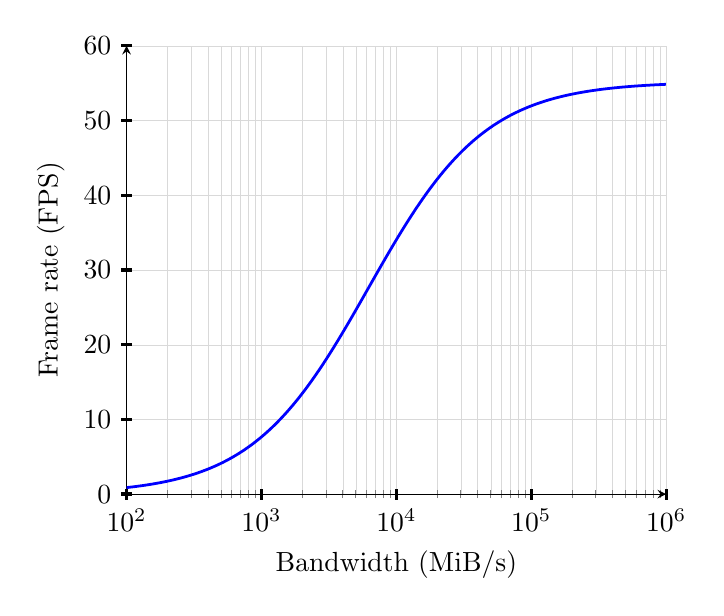
\begin{tikzpicture}
    \begin{semilogxaxis}[
        axis lines = left,
        xlabel = {Bandwidth (MiB/s)},
        ylabel = {Frame rate (FPS)},
        ymin = 0, ymax = 60,
        xmin = 100, xmax = 1000000,
        ytick distance=10,
        grid=both,
        grid style={line width=.1pt, draw=gray!30},
        legend pos={north west},
        every major tick/.append style={very thick, major tick length=4pt, black},
    ]
    
    \addplot [
        domain=1:1000000, 
        samples=1000, 
        color=blue,
        line width=1pt
    ]
    {1/( ((28.75/x) + (7.08/1000)) + ((20.06/x) + (2.65/1000)) + ((30.44/x) + (4.01/1000)) + ((17.71/x) + (2.34/1000)) + ((15.54/x) + (2.04/1000)) )};
    % \addlegendentry{TODO}
    \end{semilogxaxis}
    \end{tikzpicture}
